\documentclass[../thesis.tex]{subfiles}

\begin{document}
\vspace{-1\baselineskip}

Reconstruction software reconstructs basic objects from signals collected from the event: interaction vertices, tracks, topological clusters of energy deposits\\
These quantities then used to reconstruct physics objects i.e. particles (electron, muon), jets, MET

\section{Primary reconstruction}
\label{sec:primaryreco}

\subsection*{Topological clusters}
\label{sec:topocluster}
\citep{reco:topocluster}\citep{reco:topocluster_2}\\
Topological cluster (topo-cluster): Clusters of topologically connected cell signals in the calorimeter at the EM scale. This scale does not consider loss of signal from hadrons. Singular hits without hits from neighboring cells are considered noise.\\
Done in an effort to extract signal while minimizing electronic effects and physical fluctuations. 
Used to reconstruct hadronic objects and particles decaying hadronically i.e. $\tau$ leptons\\
Signal hits with significance above a cell signal significance level $\varsigma_\mathrm{cell}^\mathrm{EM}$ are seeded in as part of a proto-cluster. Neighboring cells satisfying a cluster growth threshold are collected into the cluster.\\
Two clusters are merged if a cell is matched to both\\
If a cluster has two or more local signal maxima satisfying $E_\mathrm{cell}^\mathrm{EM}>500$ MeV, the cluster is split accordingly.\\
The process continues iteratively until all cells with significant signal efficiency have been matched to a cluster.\\
\begin{figure}[!htbp]
\begin{center}
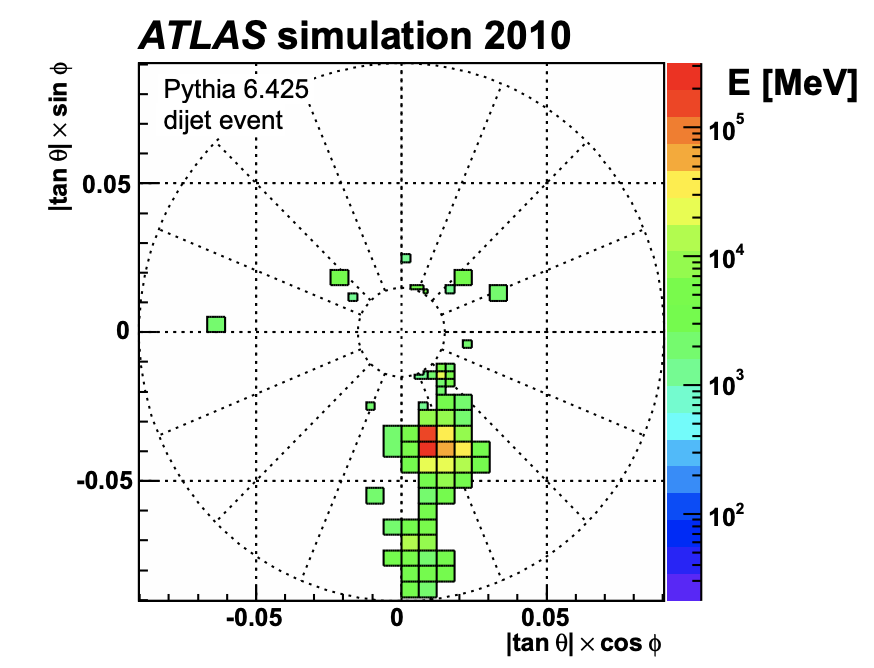
\includegraphics[width=\linewidth]{fig/reco_topo1.png}
\caption{\label{fig:reco:topo1}}
\end{center}
\end{figure}

\subsection*{Tracks}
\citep{reco:track}\\
Charged particles deposit energy in different layers of the inner detector and muon spectrometer\\
ID reco software: inside-out and outside-in algorithms\\
\begin{itemize}

\item Inside-out: \citep{reco:io}\\
Starts with seeded hits in the silicon detector in pixel \& SCT\\
Loosely matched to an EM cluster to form a track candidate\\
Hits are added to form a track candidate using a pattern recognition algorithm based on a Kalman filter formalism \citep{reco:kalman}\\
Track candidates are then fitted with a $\chi^2$ filter \citep{reco:track_chi2} and loosely matched to a fixed-sized EM cluster. Successfully matched track candidates are re-fitted with a Gaussian-sum filter (GSF) \citep{reco:track_gsf}\\
This is followed by a track scoring strategy to resolve fake tracks \& hit ambiguity between different tracks \citep{reco:track_ambiguity}\\
Extend to TRT to form final tracks, filtered by threshold $\pT > 400$ MeV.\\
\item Outside-in: \citep{reco:oi}\\
Reverse, starts with segments in TRT extending inward to silicon hits in pixel \& SCT\\
Targeting secondary tracks (decays/interactions of primary particles) or long-lived particles
\end{itemize}

\subsection*{Vertices}
Vertices: interaction or decay point\\
Primary vertex: pp interaction point\\
%Secondary vertex: secondary interaction or decay long-lived particle\\
Important for reconstruction of the hard scattering pp interaction, resulting trajectories and kinematic information of the event\\
\begin{itemize}
\item Vertex finding:\\
Uses the z-position of a track as input\\
Vertices require to have at least 2 tracks\\
Iterative $\chi^2$ algorithm evaluate track-vertex compatibility, using the track as new seed for another vertex if large discrepancy
\item Vertex fitting:\\
Adaptive multi-vertex fitter (AVF) algorithm assigns weights that depend on the track-vertex compatibility to each track to measure the probability of the track being an outlier vs inlier.\\
Vertex is then estimated by iteratively minimizing an objective function of these weights
\end{itemize}


\section{Jets}
- Quarks, gluons \& other non-color-neutral hadrons cannot be observed individually due to QCD color confinement\\
- A non-color-neutral hadron will almost immediately undergo hadronization producing a cone of color-neutral hadrons also known as a jet\\
- Jet signals can be used to reconstruct and consequently indirectly observe the original quarks/gluons the jets originated from\\
- Jet reconstruction:
\begin{itemize}
\item PFlow: energy deposited in the calorimeter systems by charged particles is removed and replaced by particle objects created with the remaining energy in the calorimeter and tracks matched to the topo-clusters. (include PFlow graphics)
\item anti-$k_t$ algorithms: sequential recombination jet algorithms
\item pile-up jets: multiple interactions associated with one bunch crossing in addition to the hard scattering of interest and reconstructed as jets in the final states. Reconstructed pile-up jets can result from   Pile-up jets are usually from soft interactions and can be distinguished with JVT algorithm using tracking information from the ID.
\item JES/JER calibration: Jet reconstruction at EM scale does not accurately account for energy from QCD interactions and needs to be calibrated to jets reconstructed at particle level. This is done via a MC-based JES calibration sequence and additional JER calibration to match jet resolution in simulation to data using dijet events.
\item reco setting: PFlow and anti-$k_t$ algorithms with radius parameter $R=0.4$, JVT applied to reconstructed jets with $\pT < 60$ GeV and $|\eta|<2.4$.
\end{itemize}
\subsection*{Flavor tagging}
- Classification of hadronic jets is an important task for many LHC analyses especially ones studying final states (Higgs decay/4top)\\
- Flavor tagging is namely interested in identifying jets containing $b$-hadrons, $c$-hadrons, $uds$-hadrons (light-jets), and hadronic decays from $\tau$.\\
- Of these, identifying $b$-jets is of particular interest due to their characteristically long lifetime ($\approx 1.5$ ps) from decay suppression by CKM factor, with a displaced secondary decay vertex and usually a tertiary vertex from $c$-hadron decays.




\subsubsection*{Efficiency calibration}
- \citep{ftag:calib}\\
- Performance of $b$-taggers are studied on MC simulated samples. However, the $b$-tagging efficiency predicted by simulation $\varepsilon_b^\mathrm{sim}$ is usually not the same as the efficiency measured in data $\varepsilon_b^\mathrm{data}$.\\
- The correction for the rate of events after applying a $b$-tagging requirement is calibrated and applied jet by jet in the form of data-to-simulation scale factors $\mathrm{SF}=\varepsilon_b^\mathrm{data}/\varepsilon_b^\mathrm{sim}$.\\
- Usage of $b$-taggers are done via four operating points (OPs), corresponding to 60\%, 70\%, 77\% and 85\% $b$-jet tagging efficiency $\varepsilon_b$ in simulated \ttbar events in order from loosest to tightest discriminant cut points.\\
- OPs are defined by selection on the tagger output to provide a pre-defined level of $\varepsilon_b$, and act as a variable trade-off between the $b$-tagging true-positive rate (efficiency) and false-positive rate (purity) \\
- (insert TPR/FPR discriminant trade-off figure)\\
\\
\\
\\
- ttbar calibration \citep{ftag:ttbar}\\
- ptrel and high pT calibration \citep{ftag:multijet}\citep{ftag:highpt}\citep{ftag:ptrel}\\
- impact parameter \verb|->| signed transverse impact parameter significance\\
- calibration results




\subsubsection*{GN2 $b$-tagging algorithm}
\begin{figure}[!htbp]
\begin{center}
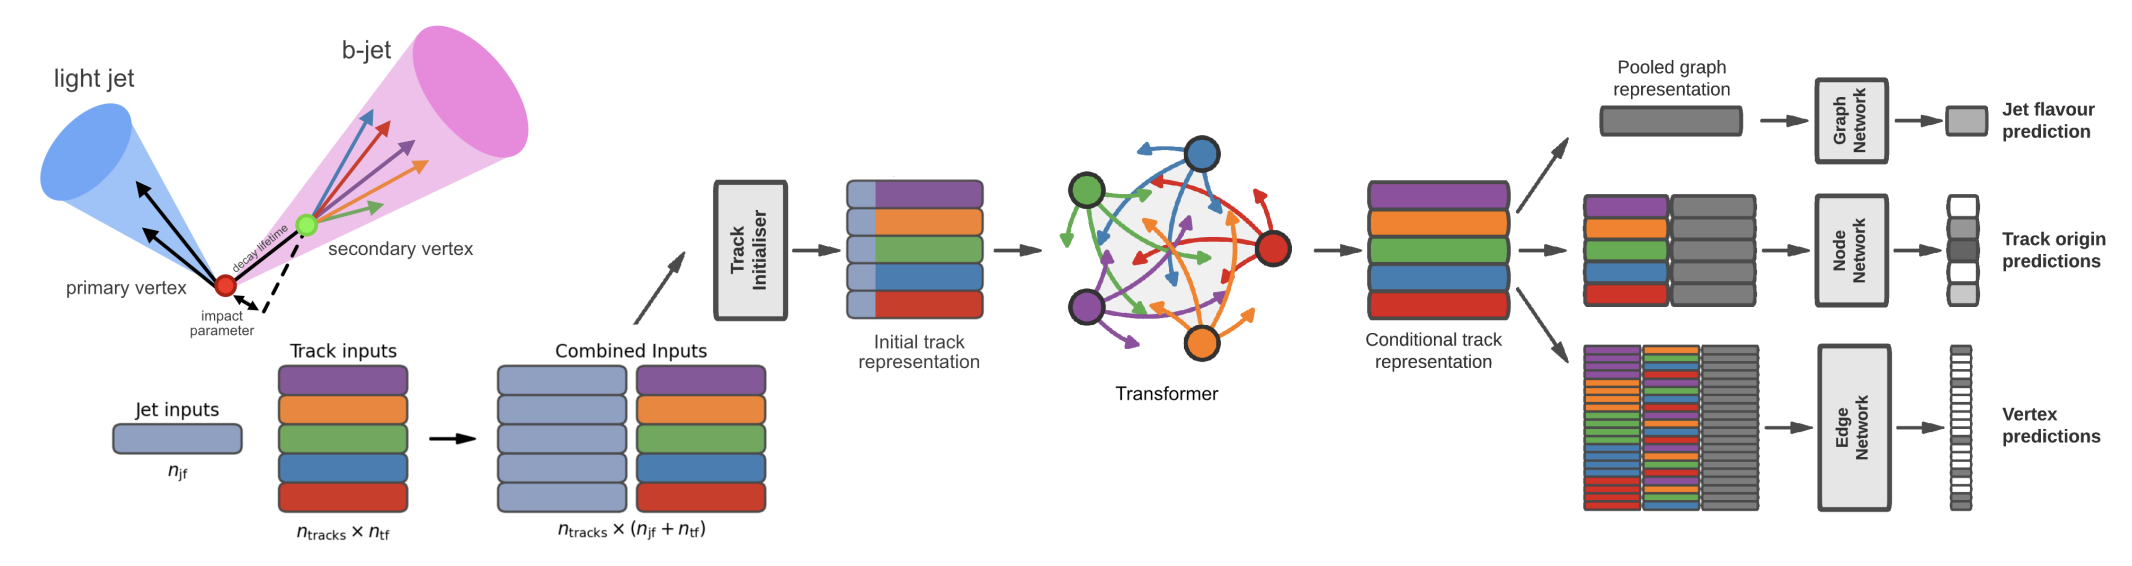
\includegraphics[width=\linewidth]{fig/ftag_gn2.png}
\caption{\label{fig:ftag:gn2} \citep{ftag:gn1}\citep{ftag:gn1.1}\citep{ftag:gn2}}
\end{center}
\end{figure}

- GN2 transformer-based $b$-tagging algorithm, utilized for analysis of Run 2 and Run 3 data\\
- GN2 gives a factor of 1.5-4 improvement in experimental applications compared to the previous convolutional neural network-based standard $b$-tagging algorithm, DL1d, without dependence on the choice of MC event generator.\\
- Attention-based architecture, modified to incorporate domain knowledge and additional auxiliary physics objectives: grouping tracks originating from common vertices and prediction of the underlying process for each track\\
- MC simulated SM \ttbar and BSM $Z'$ events from $pp$ collisions were used as training and evaluation samples. In order to minimize bias, both $b$- and light-jet samples are re-sampled to match $c$-jet distributions. \\
- GN2 concatenates 2 jet and 19 track reconstruction variables of up to 40 tracks to form the input feature vector, normalized to zero mean and unit variance.\\
- The output consists of a jet classification layer of size 4 consisting of $p_b$, $p_c$, $p_u$ and $p_\tau$ for the probability of each jet being a $b$-, $c$-, light- or $\tau$-jet respectively; a track-pairing output layer of size 2, and a track origin classification layer of 7 output categories. 

\section{Leptons}
- Lepton reconstruction is concerned mainly with electron and muon construction, since tau decays quickly and can either be reconstructed using jets or light leptons. From here on out lepton will be used mostly to refer to electrons and muons\\
- Leptons can be classified into two categories: prompt leptons resulting from heavy particle decays, or non-prompt leptons resulting from detector or reconstruction effects, or from $b$- or $c$- hadron decays\\
- Reconstruction of leptons is therefore important to study the underlying physics and suppressing background\\
\subsection{Electrons}
- \citep{reco:electron_id}\citep{reco:electron_meas}\\
- Electrons lose energy interacting with the detector materials via bremsstrahlung. The bremsstrahlung photon can then produce an electron-positron pair which can itself leaves signals in the detector, creating a collimated object that can leave multiple tracks in the ID or EM showers in the calorimeter, all considered part of the same EM topo-cluster.\\
- Electron signal signature has three characteristic components: localized energy deposits in the calorimeter, multiple tracks in the ID and compatibility between the above tracks and energy clusters in the $\eta \times \phi$ plane. Electron reconstruction in ATLAS follows these steps accordingly
\begin{figure}[!htbp]
\begin{center}
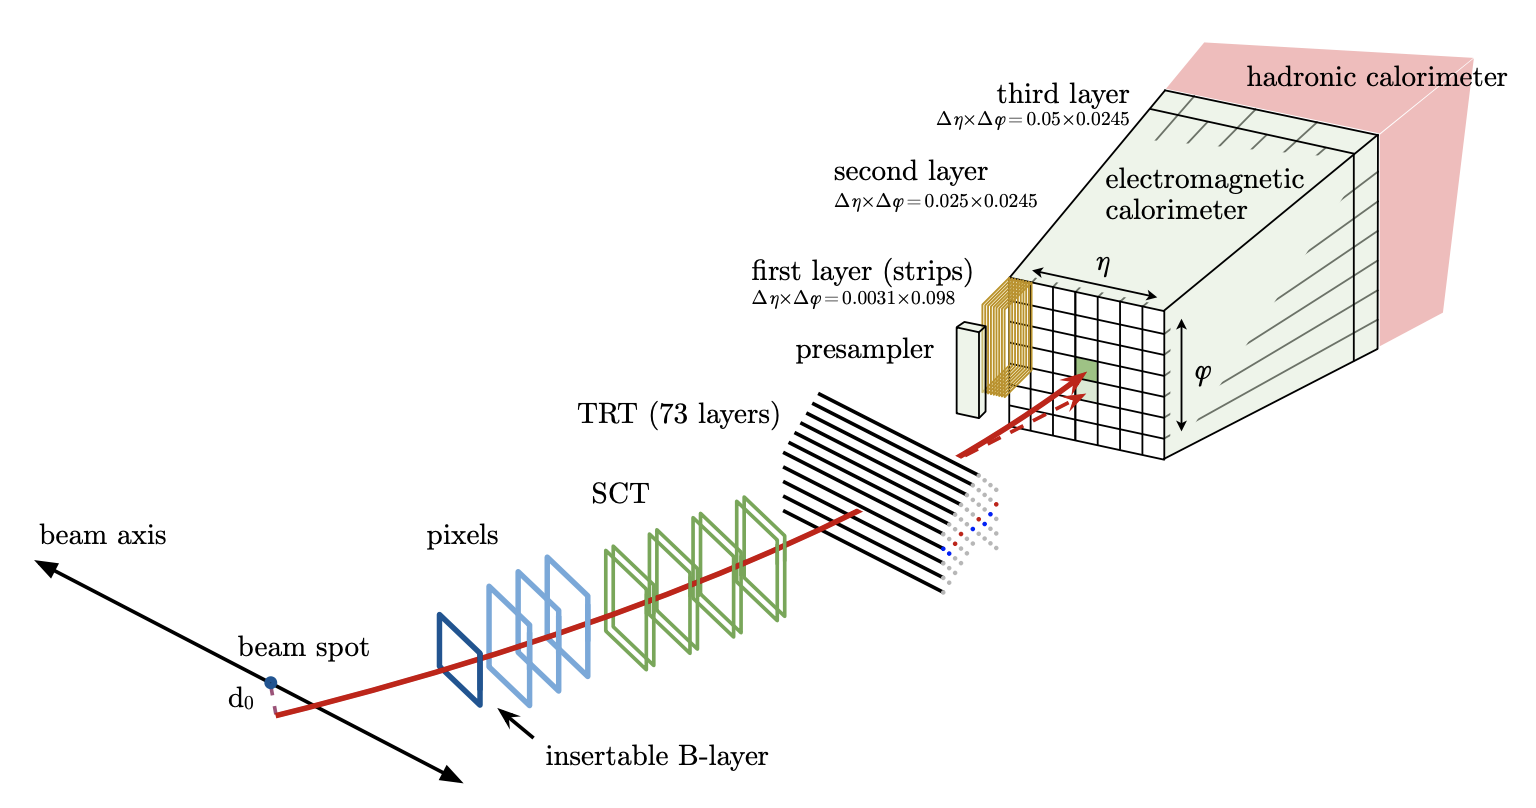
\includegraphics[width=\linewidth]{fig/reco_electron.png}
\caption{\label{fig:reco:electron}}
\end{center}
\end{figure}
- Seed-cluster reconstruction and track reconstruction are performed sequentially in accordance with the iterative clustering algorithm and track reconstruction method respectively, described in \autoref{sec:primaryreco}\\
- The seed-cluster and track candidate not associated with a conversion vertex are then matched to form an electron candidate.\\
- A reconstructed cluster is expanded from the seed-cluster in either $\phi$ or $\eta$ in the barrel or endcap region respectively\\
- The cluster energy is then calibrated to compute the original electron energy.\\




\subsection{Muons}
\section{Missing transverse momentum}
\section{Pile-up \& overlap removal}




\end{document}
